When circumventing the \gls{lvl} the code has to be modified.
There are different indicators for actual and likely modifications on the application.
Indicators for actual modifications are forced debuggability, installation from a source different than the store or the changed signature of the application.
When \textit{root} is available or \gls{luckypatcherg} is installed on a device, these are indicators for likely breaches in security.
\newline
These indicators can be tested and the program can be interrupted when in doubt.
For detected actual modifications, no reason should be given for the killing of the application, as any reason given can be used for reengineering purposes.
Indicators of an unsafe environment should trigger interruption and a dialog, explaining the risk.
Of course interruption of the application results in a bad user experience.
The tests for these indicators are implemented as seen in figure~\ref{fig:verificationNowAdditional}.
\begin{figure}[h]
    \centering
    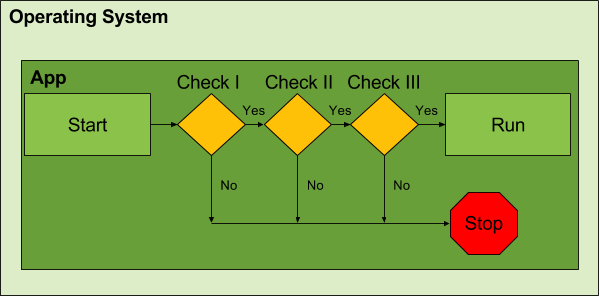
\includegraphics[width=0.8\textwidth]{data/verificationNowAdditional.png}
    \caption{Additional checks as additonal layer of security}
    \label{fig:verificationNowAdditional}
\end{figure}
\newline
Note that all these tampering countermeasures have the binary decision making, similar to the license checks process.
They can be circumvented by a reengineering effort and turning them into the unary scenario.
\newline
On reengineering, the code has to be analysed in order to find, understand and patch them.
The countermeasures should be spread inside the application to unexpectedly crash the application.
The attacker not only has to invest time to figure out why the application crashes randomly, but also to find these checks.
Obfuscation, which should be applied as a standard, makes reengineering more difficult.
\newline
None of this prevents \gls{luckypatcherg} from working, but it offers an additional layer of security.
